\begin{figure}[p]
\centering
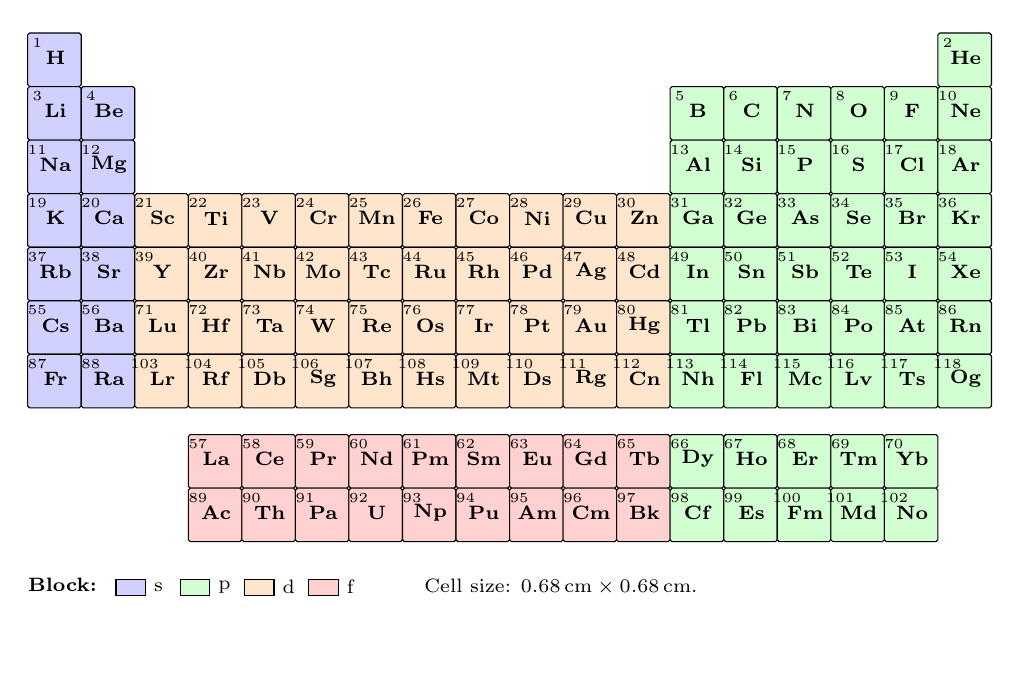
\begin{tikzpicture}[x=0.68cm, y=0.68cm, every node/.style={inner sep=0pt}]
\path[use as bounding box] (0,0.1) rectangle (18,-11.6);
\draw[fill=blue!18, draw=black, rounded corners=0.7pt] (0,0) rectangle (1,-1);
\node at (0.52,-0.46) {\scriptsize \textbf{H}};
\node at (0.18,-0.18) {\tiny 1};
\draw[fill=green!18, draw=black, rounded corners=0.7pt] (17,0) rectangle (18,-1);
\node at (17.52,-0.46) {\scriptsize \textbf{He}};
\node at (17.18,-0.18) {\tiny 2};
\draw[fill=blue!18, draw=black, rounded corners=0.7pt] (0,-1) rectangle (1,-2);
\node at (0.52,-1.46) {\scriptsize \textbf{Li}};
\node at (0.18,-1.18) {\tiny 3};
\draw[fill=blue!18, draw=black, rounded corners=0.7pt] (1,-1) rectangle (2,-2);
\node at (1.52,-1.46) {\scriptsize \textbf{Be}};
\node at (1.18,-1.18) {\tiny 4};
\draw[fill=green!18, draw=black, rounded corners=0.7pt] (12,-1) rectangle (13,-2);
\node at (12.52,-1.46) {\scriptsize \textbf{B}};
\node at (12.18,-1.18) {\tiny 5};
\draw[fill=green!18, draw=black, rounded corners=0.7pt] (13,-1) rectangle (14,-2);
\node at (13.52,-1.46) {\scriptsize \textbf{C}};
\node at (13.18,-1.18) {\tiny 6};
\draw[fill=green!18, draw=black, rounded corners=0.7pt] (14,-1) rectangle (15,-2);
\node at (14.52,-1.46) {\scriptsize \textbf{N}};
\node at (14.18,-1.18) {\tiny 7};
\draw[fill=green!18, draw=black, rounded corners=0.7pt] (15,-1) rectangle (16,-2);
\node at (15.52,-1.46) {\scriptsize \textbf{O}};
\node at (15.18,-1.18) {\tiny 8};
\draw[fill=green!18, draw=black, rounded corners=0.7pt] (16,-1) rectangle (17,-2);
\node at (16.52,-1.46) {\scriptsize \textbf{F}};
\node at (16.18,-1.18) {\tiny 9};
\draw[fill=green!18, draw=black, rounded corners=0.7pt] (17,-1) rectangle (18,-2);
\node at (17.52,-1.46) {\scriptsize \textbf{Ne}};
\node at (17.18,-1.18) {\tiny 10};
\draw[fill=blue!18, draw=black, rounded corners=0.7pt] (0,-2) rectangle (1,-3);
\node at (0.52,-2.46) {\scriptsize \textbf{Na}};
\node at (0.18,-2.18) {\tiny 11};
\draw[fill=blue!18, draw=black, rounded corners=0.7pt] (1,-2) rectangle (2,-3);
\node at (1.52,-2.46) {\scriptsize \textbf{Mg}};
\node at (1.18,-2.18) {\tiny 12};
\draw[fill=green!18, draw=black, rounded corners=0.7pt] (12,-2) rectangle (13,-3);
\node at (12.52,-2.46) {\scriptsize \textbf{Al}};
\node at (12.18,-2.18) {\tiny 13};
\draw[fill=green!18, draw=black, rounded corners=0.7pt] (13,-2) rectangle (14,-3);
\node at (13.52,-2.46) {\scriptsize \textbf{Si}};
\node at (13.18,-2.18) {\tiny 14};
\draw[fill=green!18, draw=black, rounded corners=0.7pt] (14,-2) rectangle (15,-3);
\node at (14.52,-2.46) {\scriptsize \textbf{P}};
\node at (14.18,-2.18) {\tiny 15};
\draw[fill=green!18, draw=black, rounded corners=0.7pt] (15,-2) rectangle (16,-3);
\node at (15.52,-2.46) {\scriptsize \textbf{S}};
\node at (15.18,-2.18) {\tiny 16};
\draw[fill=green!18, draw=black, rounded corners=0.7pt] (16,-2) rectangle (17,-3);
\node at (16.52,-2.46) {\scriptsize \textbf{Cl}};
\node at (16.18,-2.18) {\tiny 17};
\draw[fill=green!18, draw=black, rounded corners=0.7pt] (17,-2) rectangle (18,-3);
\node at (17.52,-2.46) {\scriptsize \textbf{Ar}};
\node at (17.18,-2.18) {\tiny 18};
\draw[fill=blue!18, draw=black, rounded corners=0.7pt] (0,-3) rectangle (1,-4);
\node at (0.52,-3.46) {\scriptsize \textbf{K}};
\node at (0.18,-3.18) {\tiny 19};
\draw[fill=blue!18, draw=black, rounded corners=0.7pt] (1,-3) rectangle (2,-4);
\node at (1.52,-3.46) {\scriptsize \textbf{Ca}};
\node at (1.18,-3.18) {\tiny 20};
\draw[fill=orange!20, draw=black, rounded corners=0.7pt] (2,-3) rectangle (3,-4);
\node at (2.52,-3.46) {\scriptsize \textbf{Sc}};
\node at (2.18,-3.18) {\tiny 21};
\draw[fill=orange!20, draw=black, rounded corners=0.7pt] (3,-3) rectangle (4,-4);
\node at (3.52,-3.46) {\scriptsize \textbf{Ti}};
\node at (3.18,-3.18) {\tiny 22};
\draw[fill=orange!20, draw=black, rounded corners=0.7pt] (4,-3) rectangle (5,-4);
\node at (4.52,-3.46) {\scriptsize \textbf{V}};
\node at (4.18,-3.18) {\tiny 23};
\draw[fill=orange!20, draw=black, rounded corners=0.7pt] (5,-3) rectangle (6,-4);
\node at (5.52,-3.46) {\scriptsize \textbf{Cr}};
\node at (5.18,-3.18) {\tiny 24};
\draw[fill=orange!20, draw=black, rounded corners=0.7pt] (6,-3) rectangle (7,-4);
\node at (6.52,-3.46) {\scriptsize \textbf{Mn}};
\node at (6.18,-3.18) {\tiny 25};
\draw[fill=orange!20, draw=black, rounded corners=0.7pt] (7,-3) rectangle (8,-4);
\node at (7.52,-3.46) {\scriptsize \textbf{Fe}};
\node at (7.18,-3.18) {\tiny 26};
\draw[fill=orange!20, draw=black, rounded corners=0.7pt] (8,-3) rectangle (9,-4);
\node at (8.52,-3.46) {\scriptsize \textbf{Co}};
\node at (8.18,-3.18) {\tiny 27};
\draw[fill=orange!20, draw=black, rounded corners=0.7pt] (9,-3) rectangle (10,-4);
\node at (9.52,-3.46) {\scriptsize \textbf{Ni}};
\node at (9.18,-3.18) {\tiny 28};
\draw[fill=orange!20, draw=black, rounded corners=0.7pt] (10,-3) rectangle (11,-4);
\node at (10.52,-3.46) {\scriptsize \textbf{Cu}};
\node at (10.18,-3.18) {\tiny 29};
\draw[fill=orange!20, draw=black, rounded corners=0.7pt] (11,-3) rectangle (12,-4);
\node at (11.52,-3.46) {\scriptsize \textbf{Zn}};
\node at (11.18,-3.18) {\tiny 30};
\draw[fill=green!18, draw=black, rounded corners=0.7pt] (12,-3) rectangle (13,-4);
\node at (12.52,-3.46) {\scriptsize \textbf{Ga}};
\node at (12.18,-3.18) {\tiny 31};
\draw[fill=green!18, draw=black, rounded corners=0.7pt] (13,-3) rectangle (14,-4);
\node at (13.52,-3.46) {\scriptsize \textbf{Ge}};
\node at (13.18,-3.18) {\tiny 32};
\draw[fill=green!18, draw=black, rounded corners=0.7pt] (14,-3) rectangle (15,-4);
\node at (14.52,-3.46) {\scriptsize \textbf{As}};
\node at (14.18,-3.18) {\tiny 33};
\draw[fill=green!18, draw=black, rounded corners=0.7pt] (15,-3) rectangle (16,-4);
\node at (15.52,-3.46) {\scriptsize \textbf{Se}};
\node at (15.18,-3.18) {\tiny 34};
\draw[fill=green!18, draw=black, rounded corners=0.7pt] (16,-3) rectangle (17,-4);
\node at (16.52,-3.46) {\scriptsize \textbf{Br}};
\node at (16.18,-3.18) {\tiny 35};
\draw[fill=green!18, draw=black, rounded corners=0.7pt] (17,-3) rectangle (18,-4);
\node at (17.52,-3.46) {\scriptsize \textbf{Kr}};
\node at (17.18,-3.18) {\tiny 36};
\draw[fill=blue!18, draw=black, rounded corners=0.7pt] (0,-4) rectangle (1,-5);
\node at (0.52,-4.46) {\scriptsize \textbf{Rb}};
\node at (0.18,-4.18) {\tiny 37};
\draw[fill=blue!18, draw=black, rounded corners=0.7pt] (1,-4) rectangle (2,-5);
\node at (1.52,-4.46) {\scriptsize \textbf{Sr}};
\node at (1.18,-4.18) {\tiny 38};
\draw[fill=orange!20, draw=black, rounded corners=0.7pt] (2,-4) rectangle (3,-5);
\node at (2.52,-4.46) {\scriptsize \textbf{Y}};
\node at (2.18,-4.18) {\tiny 39};
\draw[fill=orange!20, draw=black, rounded corners=0.7pt] (3,-4) rectangle (4,-5);
\node at (3.52,-4.46) {\scriptsize \textbf{Zr}};
\node at (3.18,-4.18) {\tiny 40};
\draw[fill=orange!20, draw=black, rounded corners=0.7pt] (4,-4) rectangle (5,-5);
\node at (4.52,-4.46) {\scriptsize \textbf{Nb}};
\node at (4.18,-4.18) {\tiny 41};
\draw[fill=orange!20, draw=black, rounded corners=0.7pt] (5,-4) rectangle (6,-5);
\node at (5.52,-4.46) {\scriptsize \textbf{Mo}};
\node at (5.18,-4.18) {\tiny 42};
\draw[fill=orange!20, draw=black, rounded corners=0.7pt] (6,-4) rectangle (7,-5);
\node at (6.52,-4.46) {\scriptsize \textbf{Tc}};
\node at (6.18,-4.18) {\tiny 43};
\draw[fill=orange!20, draw=black, rounded corners=0.7pt] (7,-4) rectangle (8,-5);
\node at (7.52,-4.46) {\scriptsize \textbf{Ru}};
\node at (7.18,-4.18) {\tiny 44};
\draw[fill=orange!20, draw=black, rounded corners=0.7pt] (8,-4) rectangle (9,-5);
\node at (8.52,-4.46) {\scriptsize \textbf{Rh}};
\node at (8.18,-4.18) {\tiny 45};
\draw[fill=orange!20, draw=black, rounded corners=0.7pt] (9,-4) rectangle (10,-5);
\node at (9.52,-4.46) {\scriptsize \textbf{Pd}};
\node at (9.18,-4.18) {\tiny 46};
\draw[fill=orange!20, draw=black, rounded corners=0.7pt] (10,-4) rectangle (11,-5);
\node at (10.52,-4.46) {\scriptsize \textbf{Ag}};
\node at (10.18,-4.18) {\tiny 47};
\draw[fill=orange!20, draw=black, rounded corners=0.7pt] (11,-4) rectangle (12,-5);
\node at (11.52,-4.46) {\scriptsize \textbf{Cd}};
\node at (11.18,-4.18) {\tiny 48};
\draw[fill=green!18, draw=black, rounded corners=0.7pt] (12,-4) rectangle (13,-5);
\node at (12.52,-4.46) {\scriptsize \textbf{In}};
\node at (12.18,-4.18) {\tiny 49};
\draw[fill=green!18, draw=black, rounded corners=0.7pt] (13,-4) rectangle (14,-5);
\node at (13.52,-4.46) {\scriptsize \textbf{Sn}};
\node at (13.18,-4.18) {\tiny 50};
\draw[fill=green!18, draw=black, rounded corners=0.7pt] (14,-4) rectangle (15,-5);
\node at (14.52,-4.46) {\scriptsize \textbf{Sb}};
\node at (14.18,-4.18) {\tiny 51};
\draw[fill=green!18, draw=black, rounded corners=0.7pt] (15,-4) rectangle (16,-5);
\node at (15.52,-4.46) {\scriptsize \textbf{Te}};
\node at (15.18,-4.18) {\tiny 52};
\draw[fill=green!18, draw=black, rounded corners=0.7pt] (16,-4) rectangle (17,-5);
\node at (16.52,-4.46) {\scriptsize \textbf{I}};
\node at (16.18,-4.18) {\tiny 53};
\draw[fill=green!18, draw=black, rounded corners=0.7pt] (17,-4) rectangle (18,-5);
\node at (17.52,-4.46) {\scriptsize \textbf{Xe}};
\node at (17.18,-4.18) {\tiny 54};
\draw[fill=blue!18, draw=black, rounded corners=0.7pt] (0,-5) rectangle (1,-6);
\node at (0.52,-5.46) {\scriptsize \textbf{Cs}};
\node at (0.18,-5.18) {\tiny 55};
\draw[fill=blue!18, draw=black, rounded corners=0.7pt] (1,-5) rectangle (2,-6);
\node at (1.52,-5.46) {\scriptsize \textbf{Ba}};
\node at (1.18,-5.18) {\tiny 56};
\draw[fill=orange!20, draw=black, rounded corners=0.7pt] (2,-5) rectangle (3,-6);
\node at (2.52,-5.46) {\scriptsize \textbf{Lu}};
\node at (2.18,-5.18) {\tiny 71};
\draw[fill=orange!20, draw=black, rounded corners=0.7pt] (3,-5) rectangle (4,-6);
\node at (3.52,-5.46) {\scriptsize \textbf{Hf}};
\node at (3.18,-5.18) {\tiny 72};
\draw[fill=orange!20, draw=black, rounded corners=0.7pt] (4,-5) rectangle (5,-6);
\node at (4.52,-5.46) {\scriptsize \textbf{Ta}};
\node at (4.18,-5.18) {\tiny 73};
\draw[fill=orange!20, draw=black, rounded corners=0.7pt] (5,-5) rectangle (6,-6);
\node at (5.52,-5.46) {\scriptsize \textbf{W}};
\node at (5.18,-5.18) {\tiny 74};
\draw[fill=orange!20, draw=black, rounded corners=0.7pt] (6,-5) rectangle (7,-6);
\node at (6.52,-5.46) {\scriptsize \textbf{Re}};
\node at (6.18,-5.18) {\tiny 75};
\draw[fill=orange!20, draw=black, rounded corners=0.7pt] (7,-5) rectangle (8,-6);
\node at (7.52,-5.46) {\scriptsize \textbf{Os}};
\node at (7.18,-5.18) {\tiny 76};
\draw[fill=orange!20, draw=black, rounded corners=0.7pt] (8,-5) rectangle (9,-6);
\node at (8.52,-5.46) {\scriptsize \textbf{Ir}};
\node at (8.18,-5.18) {\tiny 77};
\draw[fill=orange!20, draw=black, rounded corners=0.7pt] (9,-5) rectangle (10,-6);
\node at (9.52,-5.46) {\scriptsize \textbf{Pt}};
\node at (9.18,-5.18) {\tiny 78};
\draw[fill=orange!20, draw=black, rounded corners=0.7pt] (10,-5) rectangle (11,-6);
\node at (10.52,-5.46) {\scriptsize \textbf{Au}};
\node at (10.18,-5.18) {\tiny 79};
\draw[fill=orange!20, draw=black, rounded corners=0.7pt] (11,-5) rectangle (12,-6);
\node at (11.52,-5.46) {\scriptsize \textbf{Hg}};
\node at (11.18,-5.18) {\tiny 80};
\draw[fill=green!18, draw=black, rounded corners=0.7pt] (12,-5) rectangle (13,-6);
\node at (12.52,-5.46) {\scriptsize \textbf{Tl}};
\node at (12.18,-5.18) {\tiny 81};
\draw[fill=green!18, draw=black, rounded corners=0.7pt] (13,-5) rectangle (14,-6);
\node at (13.52,-5.46) {\scriptsize \textbf{Pb}};
\node at (13.18,-5.18) {\tiny 82};
\draw[fill=green!18, draw=black, rounded corners=0.7pt] (14,-5) rectangle (15,-6);
\node at (14.52,-5.46) {\scriptsize \textbf{Bi}};
\node at (14.18,-5.18) {\tiny 83};
\draw[fill=green!18, draw=black, rounded corners=0.7pt] (15,-5) rectangle (16,-6);
\node at (15.52,-5.46) {\scriptsize \textbf{Po}};
\node at (15.18,-5.18) {\tiny 84};
\draw[fill=green!18, draw=black, rounded corners=0.7pt] (16,-5) rectangle (17,-6);
\node at (16.52,-5.46) {\scriptsize \textbf{At}};
\node at (16.18,-5.18) {\tiny 85};
\draw[fill=green!18, draw=black, rounded corners=0.7pt] (17,-5) rectangle (18,-6);
\node at (17.52,-5.46) {\scriptsize \textbf{Rn}};
\node at (17.18,-5.18) {\tiny 86};
\draw[fill=blue!18, draw=black, rounded corners=0.7pt] (0,-6) rectangle (1,-7);
\node at (0.52,-6.46) {\scriptsize \textbf{Fr}};
\node at (0.18,-6.18) {\tiny 87};
\draw[fill=blue!18, draw=black, rounded corners=0.7pt] (1,-6) rectangle (2,-7);
\node at (1.52,-6.46) {\scriptsize \textbf{Ra}};
\node at (1.18,-6.18) {\tiny 88};
\draw[fill=orange!20, draw=black, rounded corners=0.7pt] (2,-6) rectangle (3,-7);
\node at (2.52,-6.46) {\scriptsize \textbf{Lr}};
\node at (2.18,-6.18) {\tiny 103};
\draw[fill=orange!20, draw=black, rounded corners=0.7pt] (3,-6) rectangle (4,-7);
\node at (3.52,-6.46) {\scriptsize \textbf{Rf}};
\node at (3.18,-6.18) {\tiny 104};
\draw[fill=orange!20, draw=black, rounded corners=0.7pt] (4,-6) rectangle (5,-7);
\node at (4.52,-6.46) {\scriptsize \textbf{Db}};
\node at (4.18,-6.18) {\tiny 105};
\draw[fill=orange!20, draw=black, rounded corners=0.7pt] (5,-6) rectangle (6,-7);
\node at (5.52,-6.46) {\scriptsize \textbf{Sg}};
\node at (5.18,-6.18) {\tiny 106};
\draw[fill=orange!20, draw=black, rounded corners=0.7pt] (6,-6) rectangle (7,-7);
\node at (6.52,-6.46) {\scriptsize \textbf{Bh}};
\node at (6.18,-6.18) {\tiny 107};
\draw[fill=orange!20, draw=black, rounded corners=0.7pt] (7,-6) rectangle (8,-7);
\node at (7.52,-6.46) {\scriptsize \textbf{Hs}};
\node at (7.18,-6.18) {\tiny 108};
\draw[fill=orange!20, draw=black, rounded corners=0.7pt] (8,-6) rectangle (9,-7);
\node at (8.52,-6.46) {\scriptsize \textbf{Mt}};
\node at (8.18,-6.18) {\tiny 109};
\draw[fill=orange!20, draw=black, rounded corners=0.7pt] (9,-6) rectangle (10,-7);
\node at (9.52,-6.46) {\scriptsize \textbf{Ds}};
\node at (9.18,-6.18) {\tiny 110};
\draw[fill=orange!20, draw=black, rounded corners=0.7pt] (10,-6) rectangle (11,-7);
\node at (10.52,-6.46) {\scriptsize \textbf{Rg}};
\node at (10.18,-6.18) {\tiny 111};
\draw[fill=orange!20, draw=black, rounded corners=0.7pt] (11,-6) rectangle (12,-7);
\node at (11.52,-6.46) {\scriptsize \textbf{Cn}};
\node at (11.18,-6.18) {\tiny 112};
\draw[fill=green!18, draw=black, rounded corners=0.7pt] (12,-6) rectangle (13,-7);
\node at (12.52,-6.46) {\scriptsize \textbf{Nh}};
\node at (12.18,-6.18) {\tiny 113};
\draw[fill=green!18, draw=black, rounded corners=0.7pt] (13,-6) rectangle (14,-7);
\node at (13.52,-6.46) {\scriptsize \textbf{Fl}};
\node at (13.18,-6.18) {\tiny 114};
\draw[fill=green!18, draw=black, rounded corners=0.7pt] (14,-6) rectangle (15,-7);
\node at (14.52,-6.46) {\scriptsize \textbf{Mc}};
\node at (14.18,-6.18) {\tiny 115};
\draw[fill=green!18, draw=black, rounded corners=0.7pt] (15,-6) rectangle (16,-7);
\node at (15.52,-6.46) {\scriptsize \textbf{Lv}};
\node at (15.18,-6.18) {\tiny 116};
\draw[fill=green!18, draw=black, rounded corners=0.7pt] (16,-6) rectangle (17,-7);
\node at (16.52,-6.46) {\scriptsize \textbf{Ts}};
\node at (16.18,-6.18) {\tiny 117};
\draw[fill=green!18, draw=black, rounded corners=0.7pt] (17,-6) rectangle (18,-7);
\node at (17.52,-6.46) {\scriptsize \textbf{Og}};
\node at (17.18,-6.18) {\tiny 118};
\draw[fill=red!18, draw=black, rounded corners=0.7pt] (3,-7.5) rectangle (4,-8.5);
\node at (3.52,-7.96) {\scriptsize \textbf{La}};
\node at (3.18,-7.68) {\tiny 57};
\draw[fill=red!18, draw=black, rounded corners=0.7pt] (4,-7.5) rectangle (5,-8.5);
\node at (4.52,-7.96) {\scriptsize \textbf{Ce}};
\node at (4.18,-7.68) {\tiny 58};
\draw[fill=red!18, draw=black, rounded corners=0.7pt] (5,-7.5) rectangle (6,-8.5);
\node at (5.52,-7.96) {\scriptsize \textbf{Pr}};
\node at (5.18,-7.68) {\tiny 59};
\draw[fill=red!18, draw=black, rounded corners=0.7pt] (6,-7.5) rectangle (7,-8.5);
\node at (6.52,-7.96) {\scriptsize \textbf{Nd}};
\node at (6.18,-7.68) {\tiny 60};
\draw[fill=red!18, draw=black, rounded corners=0.7pt] (7,-7.5) rectangle (8,-8.5);
\node at (7.52,-7.96) {\scriptsize \textbf{Pm}};
\node at (7.18,-7.68) {\tiny 61};
\draw[fill=red!18, draw=black, rounded corners=0.7pt] (8,-7.5) rectangle (9,-8.5);
\node at (8.52,-7.96) {\scriptsize \textbf{Sm}};
\node at (8.18,-7.68) {\tiny 62};
\draw[fill=red!18, draw=black, rounded corners=0.7pt] (9,-7.5) rectangle (10,-8.5);
\node at (9.52,-7.96) {\scriptsize \textbf{Eu}};
\node at (9.18,-7.68) {\tiny 63};
\draw[fill=red!18, draw=black, rounded corners=0.7pt] (10,-7.5) rectangle (11,-8.5);
\node at (10.52,-7.96) {\scriptsize \textbf{Gd}};
\node at (10.18,-7.68) {\tiny 64};
\draw[fill=red!18, draw=black, rounded corners=0.7pt] (11,-7.5) rectangle (12,-8.5);
\node at (11.52,-7.96) {\scriptsize \textbf{Tb}};
\node at (11.18,-7.68) {\tiny 65};
\draw[fill=green!18, draw=black, rounded corners=0.7pt] (12,-7.5) rectangle (13,-8.5);
\node at (12.52,-7.96) {\scriptsize \textbf{Dy}};
\node at (12.18,-7.68) {\tiny 66};
\draw[fill=green!18, draw=black, rounded corners=0.7pt] (13,-7.5) rectangle (14,-8.5);
\node at (13.52,-7.96) {\scriptsize \textbf{Ho}};
\node at (13.18,-7.68) {\tiny 67};
\draw[fill=green!18, draw=black, rounded corners=0.7pt] (14,-7.5) rectangle (15,-8.5);
\node at (14.52,-7.96) {\scriptsize \textbf{Er}};
\node at (14.18,-7.68) {\tiny 68};
\draw[fill=green!18, draw=black, rounded corners=0.7pt] (15,-7.5) rectangle (16,-8.5);
\node at (15.52,-7.96) {\scriptsize \textbf{Tm}};
\node at (15.18,-7.68) {\tiny 69};
\draw[fill=green!18, draw=black, rounded corners=0.7pt] (16,-7.5) rectangle (17,-8.5);
\node at (16.52,-7.96) {\scriptsize \textbf{Yb}};
\node at (16.18,-7.68) {\tiny 70};
\draw[fill=red!18, draw=black, rounded corners=0.7pt] (3,-8.5) rectangle (4,-9.5);
\node at (3.52,-8.96) {\scriptsize \textbf{Ac}};
\node at (3.18,-8.68) {\tiny 89};
\draw[fill=red!18, draw=black, rounded corners=0.7pt] (4,-8.5) rectangle (5,-9.5);
\node at (4.52,-8.96) {\scriptsize \textbf{Th}};
\node at (4.18,-8.68) {\tiny 90};
\draw[fill=red!18, draw=black, rounded corners=0.7pt] (5,-8.5) rectangle (6,-9.5);
\node at (5.52,-8.96) {\scriptsize \textbf{Pa}};
\node at (5.18,-8.68) {\tiny 91};
\draw[fill=red!18, draw=black, rounded corners=0.7pt] (6,-8.5) rectangle (7,-9.5);
\node at (6.52,-8.96) {\scriptsize \textbf{U}};
\node at (6.18,-8.68) {\tiny 92};
\draw[fill=red!18, draw=black, rounded corners=0.7pt] (7,-8.5) rectangle (8,-9.5);
\node at (7.52,-8.96) {\scriptsize \textbf{Np}};
\node at (7.18,-8.68) {\tiny 93};
\draw[fill=red!18, draw=black, rounded corners=0.7pt] (8,-8.5) rectangle (9,-9.5);
\node at (8.52,-8.96) {\scriptsize \textbf{Pu}};
\node at (8.18,-8.68) {\tiny 94};
\draw[fill=red!18, draw=black, rounded corners=0.7pt] (9,-8.5) rectangle (10,-9.5);
\node at (9.52,-8.96) {\scriptsize \textbf{Am}};
\node at (9.18,-8.68) {\tiny 95};
\draw[fill=red!18, draw=black, rounded corners=0.7pt] (10,-8.5) rectangle (11,-9.5);
\node at (10.52,-8.96) {\scriptsize \textbf{Cm}};
\node at (10.18,-8.68) {\tiny 96};
\draw[fill=red!18, draw=black, rounded corners=0.7pt] (11,-8.5) rectangle (12,-9.5);
\node at (11.52,-8.96) {\scriptsize \textbf{Bk}};
\node at (11.18,-8.68) {\tiny 97};
\draw[fill=green!18, draw=black, rounded corners=0.7pt] (12,-8.5) rectangle (13,-9.5);
\node at (12.52,-8.96) {\scriptsize \textbf{Cf}};
\node at (12.18,-8.68) {\tiny 98};
\draw[fill=green!18, draw=black, rounded corners=0.7pt] (13,-8.5) rectangle (14,-9.5);
\node at (13.52,-8.96) {\scriptsize \textbf{Es}};
\node at (13.18,-8.68) {\tiny 99};
\draw[fill=green!18, draw=black, rounded corners=0.7pt] (14,-8.5) rectangle (15,-9.5);
\node at (14.52,-8.96) {\scriptsize \textbf{Fm}};
\node at (14.18,-8.68) {\tiny 100};
\draw[fill=green!18, draw=black, rounded corners=0.7pt] (15,-8.5) rectangle (16,-9.5);
\node at (15.52,-8.96) {\scriptsize \textbf{Md}};
\node at (15.18,-8.68) {\tiny 101};
\draw[fill=green!18, draw=black, rounded corners=0.7pt] (16,-8.5) rectangle (17,-9.5);
\node at (16.52,-8.96) {\scriptsize \textbf{No}};
\node at (16.18,-8.68) {\tiny 102};
\node[anchor=west] at (0.0,-10.309999999999999) {\scriptsize \textbf{Block:}};
\draw[fill=blue!18, draw=black] (1.65,-10.2) rectangle (2.2,-10.5);
\node[anchor=west] at (2.3499999999999996,-10.35) {\scriptsize s};
\draw[fill=green!18, draw=black] (2.8499999999999996,-10.2) rectangle (3.3999999999999995,-10.5);
\node[anchor=west] at (3.55,-10.35) {\scriptsize p};
\draw[fill=orange!20, draw=black] (4.05,-10.2) rectangle (4.6,-10.5);
\node[anchor=west] at (4.75,-10.35) {\scriptsize d};
\draw[fill=red!18, draw=black] (5.25,-10.2) rectangle (5.8,-10.5);
\node[anchor=west] at (5.95,-10.35) {\scriptsize f};
\node[anchor=west] at (7.4,-10.35) {\scriptsize Cell size: $0.68\,\mathrm{cm}\times0.68\,\mathrm{cm}$.};
\end{tikzpicture}
\caption{Variant 0: classical periodic table used as the reference. Element positions, symbols, and positive-$Z$ indexing follow the IUPAC source basis cited in the manuscript; colors encode only the matter orbital-block structure.}
\label{fig:ptable-standard}
\end{figure}
